\documentclass{tufte-handout}

\usepackage{style}

\begin{document}

\tma{04} % TMA number

\section{Part A}

%Question 5
\begin{question}

\[ A = \{ (x,y) \in \R^{2} : 2 |x| \leq 3 \} \]

\[ B = \{ (x,y) \in \R^{2} : x^{2} + y^{2} < 4 \} \]

\[ C = A \cap B \]

    \qpart

    Sketch of set (A):

\begin{tikzpicture}[scale=1.2]
% Axes
\draw[->] (-3,0) -- (3,0) node[right] {$x$};
\draw[->] (0,-3) -- (0,3) node[above] {$y$};

% 2|x| ≤ 3 boundaries (solid)
\draw[>=stealth,->,thick, red] (-1.5,-3) -- (-1.5,3);
\draw[>=stealth,->,thick, red] ( 1.5,-3) -- ( 1.5,3);

% Labels
\node[blue] at (1.7,-0.1) {$\tfrac32$};
\node[blue] at (-1.7,-0.1) {$-\tfrac32$};

\end{tikzpicture}

\vspace{2cm}

Sketch of set (B):

\begin{tikzpicture}[scale=1.2]
% Axes
\draw[->] (-3,0) -- (3,0) node[right] {$x$};
\draw[->] (0,-3) -- (0,3) node[above] {$y$};

% Circle x^2 + y^2 < 4 (dashed)
\draw[thick, red, dashed] (0,0) circle (2);

% Labels
\node[blue] at (2.2,0) {$2$};
\node[blue] at (0,2.2) {$2$};
\node[blue] at (-2.2,0) {$-2$};
\node[blue] at (0,-2.2) {$-2$};
\end{tikzpicture}

\vspace{2cm}

    Sketch of set (C):

\begin{tikzpicture}[scale=1.2]
% Axes
\draw[->] (-3,0) -- (3,0) node[right] {$x$};
\draw[->] (0,-3) -- (0,3) node[above] {$y$};

% 2|x| ≤ 3 boundaries (solid)
\draw[>=stealth,->,thick, red] (-1.5,-3) -- (-1.5,3);
\draw[>=stealth,->,thick, red] ( 1.5,-3) -- ( 1.5,3);   

% Circle x^2 + y^2 < 4 (dashed)
\draw[thick, red, dashed] (0,0) circle (2); 

% Labels
\node[blue] at (1.7,-0.1) {$\tfrac32$};
\node[blue] at (-1.7,-0.1) {$-\tfrac32$};
\node[blue] at (2.2,0) {$2$};
\node[blue] at (0,2.2) {$2$};
\node[blue] at (-2.2,0) {$-2$};
\node[blue] at (0,-2.2) {$-2$};
\end{tikzpicture}   


Maybe

\begin{tikzpicture}[scale=1.2]
% Axes
\draw[->] (-3,0) -- (3,0) node[right] {$x$};
\draw[->] (0,-3) -- (0,3) node[above] {$y$};

% 2|x| ≤ 3 boundaries (solid)
\draw[>=stealth,->,thick, red] (-1.5,-3) -- (-1.5,3);
\draw[>=stealth,->,thick, red] ( 1.5,-3) -- ( 1.5,3);   

% CLIPPED CIRCLE: Only shows between x = -1.5 and x = 1.5
\begin{scope}
    \clip (-1.5, -2.5) rectangle (1.5, 2.5);
    \draw[thick, red, dashed] (0,0) circle (2); 
\end{scope}

% Labels
\node[blue, below] at (1.5,0) {$\tfrac32$};
\node[blue, below] at (-1.5,0) {$-\tfrac32$};
\node[blue, right] at (2,0.2) {$2$};
\node[blue, above right] at (0,2) {$2$};
\node[blue, left] at (-2,0.2) {$-2$};
\node[blue, below right] at (0,-2) {$-2$};
\end{tikzpicture}

Maybe 2

\begin{tikzpicture}[scale=1.2]
% Axes
\draw[->] (-3,0) -- (3,0) node[right] {$x$};
\draw[->] (0,-3) -- (0,3) node[above] {$y$};

% Parameters
\pgfmathsetmacro{\r}{2}
\pgfmathsetmacro{\xcut}{1.5} % = 3/2
\pgfmathsetmacro{\ycut}{sqrt(\r*\r-\xcut*\xcut)} % = sqrt(7)/2

% Shade and draw the part of the disk that lies in the vertical strip |x|<=3/2

% CLIPPED CIRCLE: Only shows between x = -1.5 and x = 1.5
\begin{scope}
      \clip (-\xcut,-\r) rectangle (\xcut,\r);
  \fill[blue!10] (0,0) circle (\r);
  \draw[thick, red, dashed] (0,0) circle (\r);
\end{scope}

% Draw ONLY the boundary segments x=±3/2 that lie inside the disk
\draw[thick, red] (-\xcut,-\ycut) -- (-\xcut,\ycut);
\draw[thick, red] ( \xcut,-\ycut) -- ( \xcut,\ycut);


% Labels
\node[blue, below] at (\xcut,0) {$\tfrac32$};
\node[blue, below] at (-\xcut,0) {$-\tfrac32$};
\node[blue, right] at (\r,0) {$2$};
\node[blue, above] at (0,\r) {$2$};
\node[blue, left] at (-\r,0) {$-2$};
\node[blue, below] at (0,-\r) {$-2$};
\end{tikzpicture}


\qpart

\qsubpart

By \textup{Definition 3.6 HB Chapter 16 p84 },

let \( x = \frac{3}{2} \) and solve for \( y \) in set B's inequality:
\[ x^{2} + y^{2} < 4 \];

then \( y = \sqrt{2^{2} - (\frac{3}{2})^{2}} = \sqrt{\frac{7}{4}} = \frac{\sqrt{7}}{2} \).
Thus, one closure point is \( (\frac{3}{2}, \frac{\sqrt{7}}{2}) \).

\qsubpart

Closure of set C is:
\[ C1 = \{ (x,y) \in \R^{2} : 2|x| \leq 3 \text{ and } x^{2} + y^{2} \leq 4 \} \]

\bigskip

Interior of set C is:
\[ Int = \{ (x,y) \in \R^{2} : 2|x| < 3 \text{ and } x^{2} + y^{2} < 4 \} \]

\bigskip

Boundary of set C is:
\[ Bd = \{ (x,y) \in \R^{2} : (2|x| = 3 \text{ and } x^{2} + y^{2} \leq 4) \text{ or } (2|x| \leq 3 \text{ and } x^{2} + y^{2} = 4) \} \]

\vspace{2cm}

\qpart

Given the 'mixed' metric \( d \);

\[ d((x_{1},y_{1}),(x_{2},y_{2})) = |x_{1} - x_{2}| + d_{0}(y_{1},y_{2}) \]

By \textup{Definition 2.3 HB Chapter 14 p72}

Where \( d_{0} \) is the discrete metric defined on \( \R \)
\[ d_{0}(y_{1},y_{2}) = \begin{cases}
0, \text{ if } y_{1} = y_{2},\\
1, \text{ if } y_{1} \neq y_{2}.
\end{cases} \]

As \( y_{1} \neq y_{2} \) for all points in set C,

then \( d_{0}(y_{1},y_{2}) = 1 \).

Thus,
\[ d((x_{1},y_{1}),(x_{2},y_{2})) = |x_{1} - x_{2}| + 1 \]







\end{question}

\end{document}